\vfill\eject
\section{Implementation}
\label{sec:implement}
In this section we first attempt to experimentally determine the value for
paramaters in our framework and then describe a baseline system for comparison
with our framework.
\subsection{Taxonomy}
There are more than 37000 tags in {\it Stack overflow} nowadays. A large part
of them are not used frequently and many of them share very close meanings.
We eliminate the tag graph by removing tags with a frequency less than 50 posts.
The clustering method we used is {\it K-means} with $k=20$. Afer this is done,
we extract more than 500,000 post from {\it Stack overflow} to train the taxonomy
system. We use Labeled LDA from Stanford Topic Modeling Toolbox.
%\begin{figure}[h]
%\centering
%\label{fig:labelperdoc}
%\epsfig{file=figure/freq_dist_1.eps,width=0.7\columnwidth}
%\caption{Number of documents that have $L$ labels}
%\end{figure}

%\begin{figure}[h]
%\centering
%\label{fig:docperlabel}
%\epsfig{file=figure/freq_dist_2.eps,width=0.7\columnwidth}
%\caption{Number of labels that appear in $D$ documents}
%\end{figure}

\subsection{Parameter Settings}
\label{sec:config}
We set the three parameters in our model, namely, $K$: the number
of topics, $\lambda$ : the weight of $p(w|z)$, and $\eta$ : the weight of $p(w|z)$, by
tuning them one by one on the development set.

\begin{figure}[h]
\begin{center}
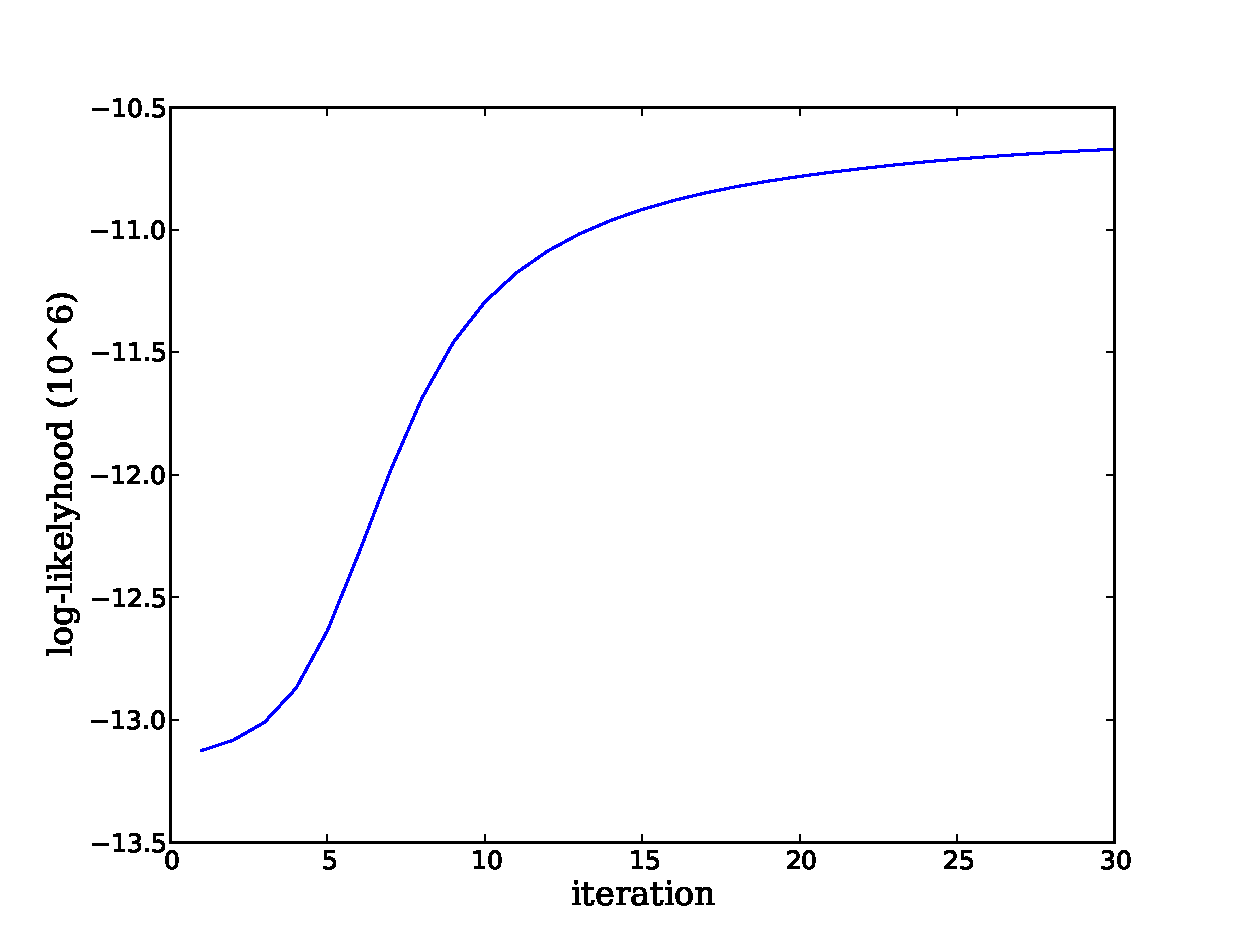
\includegraphics[width=0.7\columnwidth]{figure/likelyhood.eps}
\caption{Convergence parameters}
\label{fig:conv}
\end{center}
\end{figure}
\subsection{Baseline System}
We build two baseline systems to test the code mining performance.
\subsubsection{``TF-IDF$+$SVM''}
For this system, we use the words distributions to evaluate the relationships
between source code files and the tags. The tag taxonomy is build with
{\it Support Vector Machine}
\subsubsection{``LDA$+$Labeled-LDA''}
To evaluate the effectiveness of our repository model, we set up this baseline
system by applying LDA model to repositories without considering the structure
of them.

